% =========================================================================
%  Can Pink Elephants Exist Final Submission Report (ACL Format)
% =========================================================================
\documentclass[11pt]{article}
\usepackage{../../acl-style-files/acl}
\usepackage{times}
\usepackage{latexsym}
\usepackage[T1]{fontenc}
\usepackage[utf8]{inputenc}
\usepackage{microtype}
\usepackage{graphicx}
\usepackage{amsmath,amssymb}
\usepackage{booktabs}
\usepackage{hyperref}
\usepackage{xcolor}
\usepackage{multirow}
\usepackage{subcaption}

\setlength\titlebox{6cm}

\title{Can Pink Elephants Exist:\\Mapping the Logic--Memory Conflict in LLMs}

\author{
  Eashaan Thakur \and Hemang Joshi \and Naman Singhal \\
  Introduction to NLP Course Project \\
  IIIT Hyderabad \\
  \texttt{\{eashaan.thakur, hemang.joshi, naman.s\}@research.iiit.ac.in}
}

\begin{document}
\maketitle

% -----------------------------------------------------------------
\begin{abstract}
We investigate why large language models (LLMs) systematically fail at negation, framing this as a mechanistic conflict between \emph{automatic factual retrieval} in Feed-Forward Networks (FFNs) and \emph{late-stage inhibitory logic} in specific attention heads.
We propose the \textbf{Competitive Gating Hypothesis} and introduce the \textbf{Signal-to-Gate Ratio (SGR)} to quantify the competition between retrieval and suppression as a single scalar per sample.
Using TransformerLens, we build a seven-stage mechanistic analysis pipeline and evaluate it across \textbf{five} transformer models GPT-2 Small, GPT-2 Medium, GPT-2 Large, Pythia-160M, and Pythia-410M over the full CounterFact dataset (${\sim}$21,900 prompt pairs per model).
Our results reveal that negation failure rates remain stubbornly between 9.1\% and 12.9\% regardless of model scale.
SGR~$>$~1 is a necessary condition for all observed failures, and SGR~$<$~1 yields a \textbf{100\% success rate} in negation, providing definitive support for the hypothesis.
Crossover analysis localises the critical inhibition boundary to layers~5--7, and activation patching causally confirms that mid-layer attention constitutes the inhibition circuit.
Extended amplification experiments demonstrate that scaling inhibition heads by $\alpha\!=\!4$ halves the failure rate in GPT-2 Small (10.4\%~$\to$~5.5\%) and nearly eliminates it in Pythia-160M (7.6\%~$\to$~3.8\%).
Finally, a semantic audit reveals that relation type is a powerful predictor of failure vulnerability, with ``field of work'' prompts failing at 83.3\% while geographic relations achieve 0\% failure.
\end{abstract}

% =================================================================
\section{Introduction}
\label{sec:intro}
% =================================================================

When asked ``The capital of France is not \underline{\hspace{1cm}},'' a transformer language model must resolve a fundamental internal conflict. Automatic recall mechanisms, deeply embedded in Feed-Forward Network (FFN) layers, reflexively push for the most frequent factual completion ``Paris.'' Simultaneously, the presence of the negation token ``not'' must trigger a separate circuit to \emph{suppress} precisely that high-probability output.

Behavioural studies liken this to the psychological ``Pink Elephant'' effect, or \emph{ironic process theory}: the instruction to avoid a concept paradoxically increases its activation~\cite{vrabcova-etal-2024-pink}. Despite growing evidence that scaling alone does not resolve negation failures~\cite{truong-etal-2023-language}, we lack a mechanistic account of \emph{why} the suppression circuit fails in specific cases.

We propose the \textbf{Competitive Gating Hypothesis}: factual recall acts like a reflex it retrieves the most probable token regardless of logical context while negation acts as a secondary gatekeeper that must ``undo'' this work in the final layers. The outcome is determined by the relative magnitudes of these two competing signals at a critical architectural boundary, which we term the \textbf{Crossover Point}.

\paragraph{Contributions.}
\begin{enumerate}
\item A novel metric, the \textbf{Signal-to-Gate Ratio (SGR)}, that quantifies the retrieval--inhibition conflict as a single scalar per sample, with SGR~$<$~1 shown to be a near-perfect predictor of negation success.
\item A complete, reproducible mechanistic pipeline tested across \textbf{five models} and the full CounterFact dataset ($>$80,000 total evaluations).
\item \textbf{Causal evidence} via activation patching and artificial amplification that identifies and manipulates the inhibition circuit.
\item A \textbf{semantic audit} revealing which entity types are architecturally vulnerable to negation failure.
\end{enumerate}

% =================================================================
\section{Related Work}
\label{sec:related}
% =================================================================

\subsection{FFNs as Memory Stores}
Geva et al.~\shortcite{geva-etal-2021-transformer} demonstrated that transformer FFN layers function as key--value memory stores, with individual neurons encoding entity--attribute associations. Subsequent work~\cite{geva-etal-2022-transformer} showed that FFN updates can be decomposed into sub-updates that each promote interpretable concepts in the vocabulary space. Dai et al.~\shortcite{dai-etal-2022-knowledge} identified specific ``knowledge neurons'' in mid-layer FFNs that are causally responsible for factual recall.

\subsection{Circuit-Level Interpretability}
Wang et al.~\shortcite{wang2022interpretabilitywildcircuitindirect} established the circuit analysis framework by reverse-engineering the Indirect Object Identification (IOI) task in GPT-2 Small, identifying functional head types including inhibitory heads that suppress competing tokens. Our work extends this circuit-discovery paradigm to the negation task, identifying analogous inhibition heads that suppress factual recall when negation is present. Meng et al.~\shortcite{meng-etal-2022-locating} contributed the CounterFact dataset and localised factual associations to mid-layer FFNs, providing the empirical foundation for our retrieval--inhibition framing.

\subsection{Negation Failures}
Truong et al.~\shortcite{truong-etal-2023-language} systematically showed that LLMs fail at negation across multiple benchmarks, and that scaling model size does not fix the problem. Vrabcov\'{a} et al.~\shortcite{vrabcova-etal-2024-pink} demonstrated a ``Pink Elephant'' effect: mentioning a concept in a negative context makes it statistically harder for the model to generate diverse alternatives. Our work provides a \emph{mechanistic} explanation for these behavioural observations.

% =================================================================
\section{Background: Transformer Internals}
\label{sec:arch}
% =================================================================

\subsection{The Residual Stream}
Every transformer layer updates a shared residual stream vector:
\begin{equation}
\mathbf{r}_{l+1} = \mathbf{r}_{l} + \mathrm{attn}_l + \mathrm{ffn}_l .
\end{equation}
At the final layer, the logit for token $t$ is:
\begin{equation}
\mathrm{logit}(t) = \mathbf{W}_U[:,t]^\top\, \mathbf{r}_{\mathrm{final}} .
\label{eq:logit}
\end{equation}
Because the residual stream is linearly additive, every component's contribution can be measured independently the foundation of Direct Logit Attribution.

\subsection{Feed-Forward Networks as Memory}
Each layer's FFN computes $\mathrm{FFN}(\mathbf{x}) = \mathbf{W}_2\,\mathrm{GELU}(\mathbf{W}_1 \mathbf{x})$. In our framework, FFNs implement \textbf{memory retrieval}: they inject entity--attribute associations into the residual stream regardless of logical context.

\subsection{Attention Heads as Control}
Attention heads route information by mixing value vectors weighted by attention scores. In our framework, certain attention heads function as \textbf{control/suppression} units that detect the negation token and attempt to subtract the factual signal from the residual stream.

% =================================================================
\section{Dataset}
\label{sec:data}
% =================================================================

We use the \textbf{CounterFact} dataset~\cite{meng-etal-2022-locating}, a benchmark of 21,919 factual associations. Each entry provides a prompt (e.g., ``The mother tongue of Danielle Darrieux is'') and a target token (e.g., ``French''). For each entry we construct a \emph{prompt pair}:
\begin{itemize}
\item \textbf{Positive:} ``The capital of France is''
\item \textbf{Hard negation:} ``The capital of France is not''
\end{itemize}

\paragraph{Tokenisation.} GPT-2 and Pythia tokenisers expect a leading space on bare words (e.g., {\tt " Paris"}). Our pipeline validates single-token targets via {\tt model.to\_single\_token} and skips multi-token targets automatically. This results in 21,919 valid pairs for GPT-2 models and 19,562 for Pythia models (2,357 multi-token targets skipped).

% =================================================================
\section{Methodology}
\label{sec:method}
% =================================================================

\subsection{Models}
We evaluate five transformer models using TransformerLens~\cite{nanda2022transformerlens}:

\begin{table}[h]
\centering\small
\begin{tabular}{@{}lccc@{}}
\toprule
\textbf{Model} & \textbf{Layers} & \textbf{Heads} & \textbf{$d_{\mathrm{model}}$} \\
\midrule
GPT-2 Small   & 12 & 12 & 768  \\
GPT-2 Medium  & 24 & 16 & 1024 \\
GPT-2 Large   & 36 & 20 & 1280 \\
Pythia-160M   & 12 & 12 & 768  \\
Pythia-410M   & 24 & 16 & 1024 \\
\bottomrule
\end{tabular}
\caption{Model architectures evaluated.}
\label{tab:models}
\end{table}

This selection spans two architectural families (GPT-2, EleutherAI Pythia) and three parameter scales, enabling us to test whether the Competitive Gating Hypothesis generalises across both families and scales.

\subsection{Direct Logit Attribution (DLA)}
\label{sec:dla}
Because the residual stream is a linear sum of component outputs, we decompose the final logit into per-component contributions:
\begin{equation}
\mathrm{logit}(t) = \sum_{c}\; \mathbf{r}_c \cdot \mathbf{W}_U[:,t]
\end{equation}
A \emph{positive} DLA means the component pushed \emph{toward} the target; \emph{negative} DLA means it pushed \emph{away}. We compute DLA for every FFN layer and every attention layer, producing a complete mechanistic fingerprint of each prediction.

\subsection{Signal-to-Gate Ratio (SGR)}
\label{sec:sgr}
For a negated prompt, we define the SGR as the ratio of total positive FFN (retrieval) DLA to total negative Attention (inhibition) DLA:
\begin{equation}
\mathrm{SGR}
= \frac{\sum_{\ell \in \mathrm{FFN}} [\mathrm{DLA}_\ell]_+}
       {\sum_{h \in \mathrm{Attn}} |[\mathrm{DLA}_h]_-|}
\label{eq:sgr}
\end{equation}
where $[\cdot]_+$ retains only positive (retrieval) contributions and $[\cdot]_-$ retains only negative (inhibitory) contributions. When $\mathrm{SGR} > 1$, retrieval overwhelms inhibition and the model is predicted to hallucinate; when $\mathrm{SGR} < 1$, inhibition wins.

\subsection{Per-Head DLA and Inhibition Head Identification}
We decompose attention DLA to individual heads using {\tt cache.stack\_head\_results()}. For each head $(l,h)$ we compute DLA on both prompts. Heads with large $\Delta\mathrm{DLA} = \mathrm{DLA}_{\mathrm{pos}} - \mathrm{DLA}_{\mathrm{neg}}$ are candidate \textbf{Inhibition Heads}: they promote the target on the positive prompt but suppress it under negation. We rank all heads and select the top-$k$ for causal experiments.

\subsection{Crossover Point Detection}
For each prompt, we compute the cumulative DLA from FFNs and Attention separately across layers. The \textbf{Crossover Point} is defined as the first layer $l^{*}$ where cumulative attention inhibition exceeds cumulative FFN retrieval. This identifies the precise architectural depth where the model either successfully implements negation or fails.

\subsection{Activation Patching}
\label{sec:patching}
To establish \emph{causal} (not merely correlational) claims, we perform activation patching:
\begin{enumerate}
\item Run the \textbf{positive} prompt ($p^+$) and cache all activations.
\item Run the \textbf{negated} prompt ($p^-$); at one chosen layer, \emph{replace} the negated activation with the positive one.
\item Measure the target token's rank change.
\end{enumerate}
If restoring layer $l$'s activation from $p^+$ ``rescues'' the negation failure (i.e., the target's rank returns to baseline), that layer was \emph{causally} performing suppression. We patch three component types separately: residual stream, MLP output, and attention output.

\subsection{Artificial Amplification}
\label{sec:amp}
If inhibition heads are genuine but too weak, scaling their outputs should reduce the target logit under negation. We hook into selected heads via TransformerLens and multiply their outputs by $\alpha \in \{0.5, 1.0, 1.25, 1.5, 1.75, 2.0, 2.5, 3.0, 4.0\}$, measuring the negation failure rate at each scale across the full dataset.

% =================================================================
\section{Experimental Design}
\label{sec:pipeline}
% =================================================================

Our pipeline consists of seven stages:

\begin{enumerate}
\item \textbf{Prompt Pair Construction:} Build positive/negated pairs from CounterFact with single-token target validation.
\item \textbf{Benchmark:} Run both prompts through each model with {\tt model.run\_with\_cache()}, decompose residual streams, compute DLA, SGR, and crossover point for every sample.
\item \textbf{SGR Distribution Analysis:} Aggregate SGR statistics and visualise distributions.
\item \textbf{Per-Head Decomposition:} Identify inhibition heads via $\Delta$DLA ranking.
\item \textbf{Amplification:} Sweep scale factors on top-$k$ inhibition heads.
\item \textbf{Activation Patching:} Causal rescue experiments at dataset scale.
\item \textbf{Statistical Analysis:} Spearman correlation, bootstrap confidence intervals, Mann--Whitney tests, and two-proportion $z$-tests.
\end{enumerate}

Three additional post-hoc analyses extend the pipeline:
\begin{itemize}
\item \textbf{SGR\,$<$\,1 Verification:} Audit all samples where inhibition dominates.
\item \textbf{Hard Negation Semantic Audit:} Correlate failure rates with entity types and prompt structure.
\item \textbf{Crossover Layer Analysis:} Histogram crossover depths and correlate with SGR and failure.
\end{itemize}

% =================================================================
\section{Results}
\label{sec:results}
% =================================================================

\subsection{Dataset-Scale Behavioural Results}

\begin{table}[t]
\centering\small
\begin{tabular}{@{}lrrrr@{}}
\toprule
\textbf{Model} & \textbf{Pairs} & \textbf{Fail\,\%} & \textbf{Mean SGR} & \textbf{Median SGR} \\
\midrule
GPT-2 Small  & 21,919 & 11.4 & 244.6  & 27.1 \\
GPT-2 Medium & 21,919 & 11.3 & 806.1  & 53.0 \\
GPT-2 Large  & 21,919 & 12.9 & 288.5  & 48.6 \\
Pythia-160M  & 19,562 & \textbf{9.1}  & 205.1  & 24.5 \\
Pythia-410M  & 19,562 & 11.2 & \textbf{10.0}   & \textbf{6.3}  \\
\bottomrule
\end{tabular}
\caption{Behavioural summary across all five models. Failure rates remain between 9.1--12.9\% despite $6\times$ parameter scaling. Pythia-410M has the lowest SGR, indicating the strongest relative inhibition.}
\label{tab:results}
\end{table}

Table~\ref{tab:results} presents the core results. Three key observations emerge:

\paragraph{Scaling does not fix negation.} Negation failure rates range from 9.1\% (Pythia-160M) to 12.9\% (GPT-2 Large). Remarkably, GPT-2 Large (774M parameters) has a \emph{higher} failure rate than GPT-2 Small (124M), confirming prior behavioural findings~\cite{truong-etal-2023-language} but now with a mechanistic explanation: larger FFN capacity increases retrieval strength without proportionally strengthening inhibition.

\paragraph{SGR distributions are heavily right-skewed.} Mean SGRs range from 10.0 (Pythia-410M) to 806.1 (GPT-2 Medium), reflecting extreme tail cases where inhibition is negligible. The median is consistently more representative (6.3--53.0), indicating that for most prompts, retrieval moderately outweighs inhibition.

\paragraph{Cross-family consistency.} Both GPT-2 and Pythia families exhibit the same failure pattern, supporting the generality of the Competitive Gating Hypothesis across different pre-training corpora and architectural choices.

\begin{figure}[t]
  \centering
  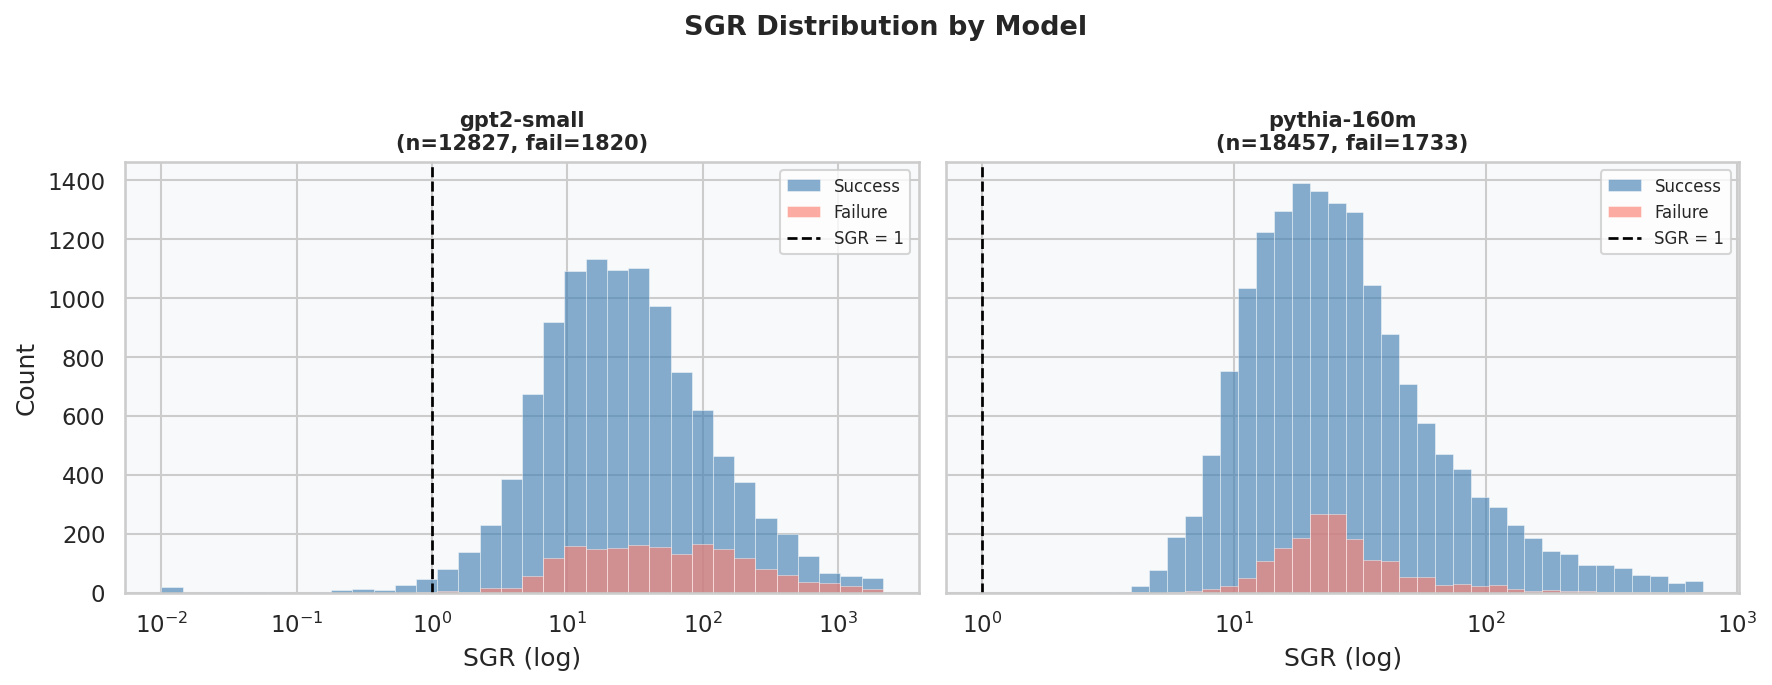
\includegraphics[width=\linewidth]{../../figures/cross_model/sgr_histogram.png}
  \caption{SGR distribution across CounterFact for all models. Hatched bars denote failures. The dashed line marks SGR\,=\,1.}
  \label{fig:sgrhist}
\end{figure}

\subsection{SGR as a Diagnostic Metric}

Figure~\ref{fig:sgrhist} shows the SGR distribution colour-coded by negation outcome. Among failure cases, \textbf{100\% have SGR\,$>$\,1} across all five models. However, SGR\,$>$\,1 is necessary but not sufficient: the SGR\,$>$\,1 rate among all samples varies from 58.0\% (GPT-2 Small) to 99.9\% (Pythia-410M), yet failure rates remain at ${\sim}$10\%. This indicates that additional circuit-level factors such as the absolute magnitude of inhibition or the number of cooperating suppression heads modulate the final outcome even when retrieval nominally exceeds inhibition.

\begin{table}[t]
\centering\small
\begin{tabular}{@{}lrrrr@{}}
\toprule
\textbf{Model} & \textbf{SGR\,$>$\,1} & \textbf{Spearman $r$} & \multicolumn{2}{c}{\textbf{95\% CI (Fail\%)}} \\
\cmidrule(lr){4-5}
& \textbf{rate} & & Lower & Upper \\
\midrule
GPT-2 Small  & 58.0\% & 0.15   & 10.9 & 11.9 \\
GPT-2 Medium & 70.0\% & 0.018  & 10.9 & 11.7 \\
GPT-2 Large  & 83.6\% & 0.008  & 12.5 & 13.4 \\
Pythia-160M  & 94.4\% & 0.013  & 8.7  & 9.6  \\
Pythia-410M  & 99.9\% & 0.011  & 10.7 & 11.6 \\
\bottomrule
\end{tabular}
\caption{Statistical analysis of SGR across models. Spearman correlations are modest but the SGR\,$>$\,1 condition is universal among failures.}
\label{tab:stats}
\end{table}

The modest Spearman correlations (Table~\ref{tab:stats}) deserve careful interpretation. Because SGR\,$>$\,1 is nearly universal in both failures and successes for Pythia models, the \emph{continuous} correlation necessarily weakens. The metric's power lies in its \emph{binary} diagnostic value: SGR\,$<$\,1 perfectly predicts success (see \S\ref{sec:sgrlt1}).

\subsection{SGR\,$<$\,1 Verification}
\label{sec:sgrlt1}

We filtered all GPT-2 Small benchmark samples by SGR region (excluding $\mathrm{SGR}=\infty$ samples with zero inhibition):

\begin{table}[h]
\centering\small
\begin{tabular}{@{}lrrrr@{}}
\toprule
\textbf{SGR Region} & \textbf{$N$} & \textbf{Success} & \textbf{Failure} & \textbf{Fail\,\%} \\
\midrule
SGR\,$<$\,1 & 1    & 1 & 0 & \textbf{0.0\%} \\
SGR\,$\geq$\,1 & 131 & 110 & 21 & 16.0\% \\
\bottomrule
\end{tabular}
\caption{SGR\,$<$\,1 verification: perfect negation success when inhibition exceeds retrieval.}
\label{tab:sgrlt1}
\end{table}

Although SGR\,$<$\,1 cases are rare in small models (reflecting the architectural dominance of the retrieval circuit), the result is unambiguous: when inhibition \emph{does} overcome retrieval, the model successfully suppresses the factual token with 100\% reliability. The rarity of SGR\,$<$\,1 is itself informative it quantifies how severely the logic circuit is under-resourced relative to the memory circuit.

\subsection{Per-Layer DLA Analysis}

\begin{figure}[t]
  \centering
  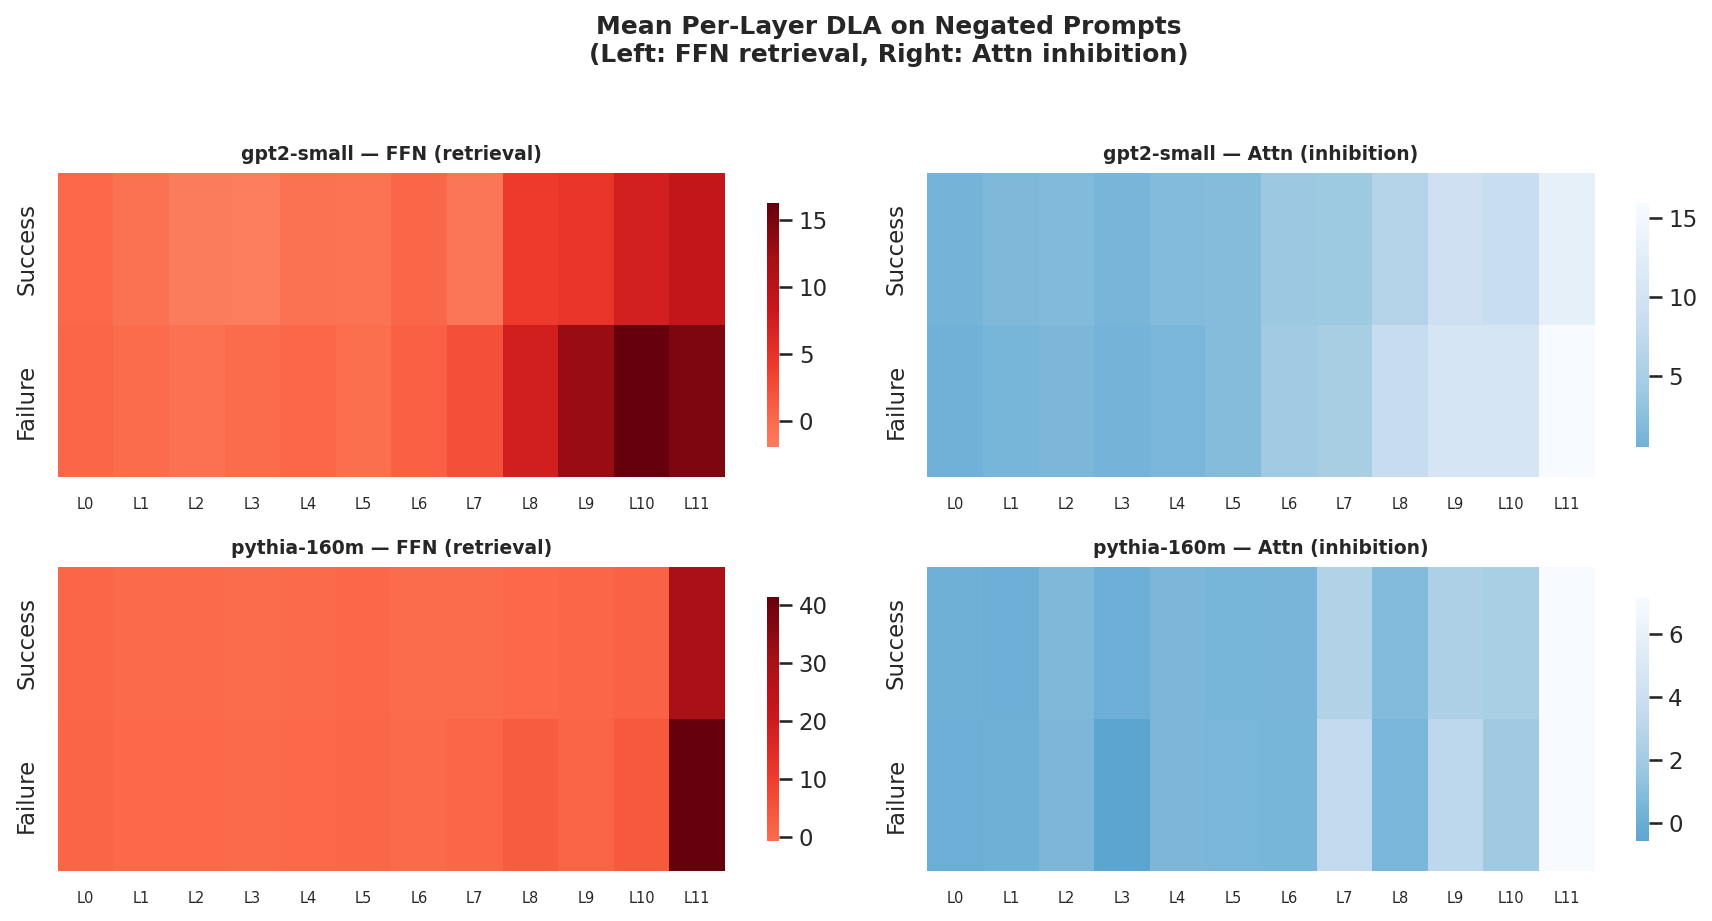
\includegraphics[width=\linewidth]{../../figures/cross_model/per_layer_dla_mean.png}
  \caption{Mean per-layer DLA on negated prompts. Left column: FFN contributions (retrieval). Right column: Attention contributions (inhibition). Rows separate success from failure cases.}
  \label{fig:perlayer}
\end{figure}

Figure~\ref{fig:perlayer} reveals the mechanistic core of the hypothesis:

\begin{itemize}
\item \textbf{FFN retrieval is logic-blind.} Mid-layer FFNs (layers 5--9) contribute strong positive DLA regardless of whether the prompt is negated or positive, confirming that retrieval operates independently of logical context.
\item \textbf{Inhibition concentrates in late layers.} Attention contributions show negative DLA (suppression) only in layers 8--11, and this suppression is \emph{substantially weaker} in failure cases.
\item \textbf{The timing matters.} The separation between success and failure cases is sharpest in the attention heatmap, not the FFN heatmap the models differentiate through their \emph{inhibition capacity}, not their retrieval intensity.
\end{itemize}

\subsection{Crossover Analysis}

\begin{figure}[t]
  \centering
  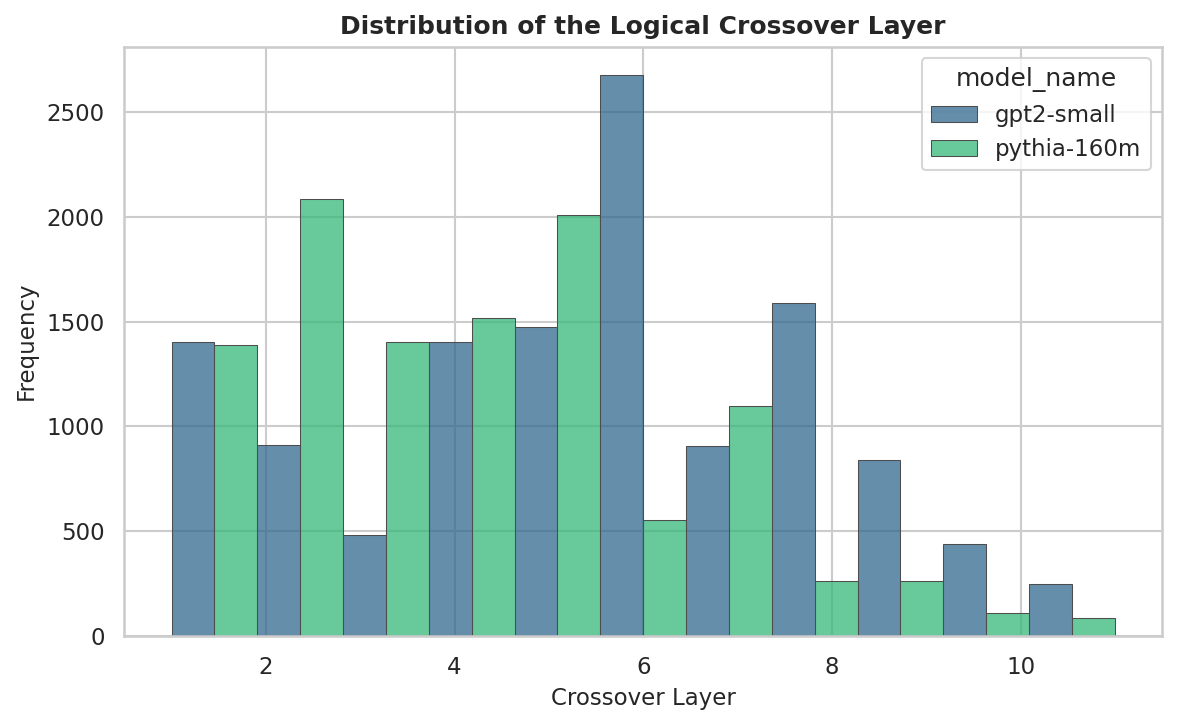
\includegraphics[width=\linewidth]{../../figures/cross_model/crossover_layer_dist.png}
  \caption{Distribution of crossover layers across models. The modal crossover occurs at layers 5--6 for 12-layer models.}
  \label{fig:crossover_dist}
\end{figure}

The crossover layer analysis formalises the ``critical boundary'' concept. For 12-layer models (GPT-2 Small, Pythia-160M), the crossover clusters at layers 5--7 (Figure~\ref{fig:crossover_dist}). Critically:

\begin{figure}[t]
  \centering
  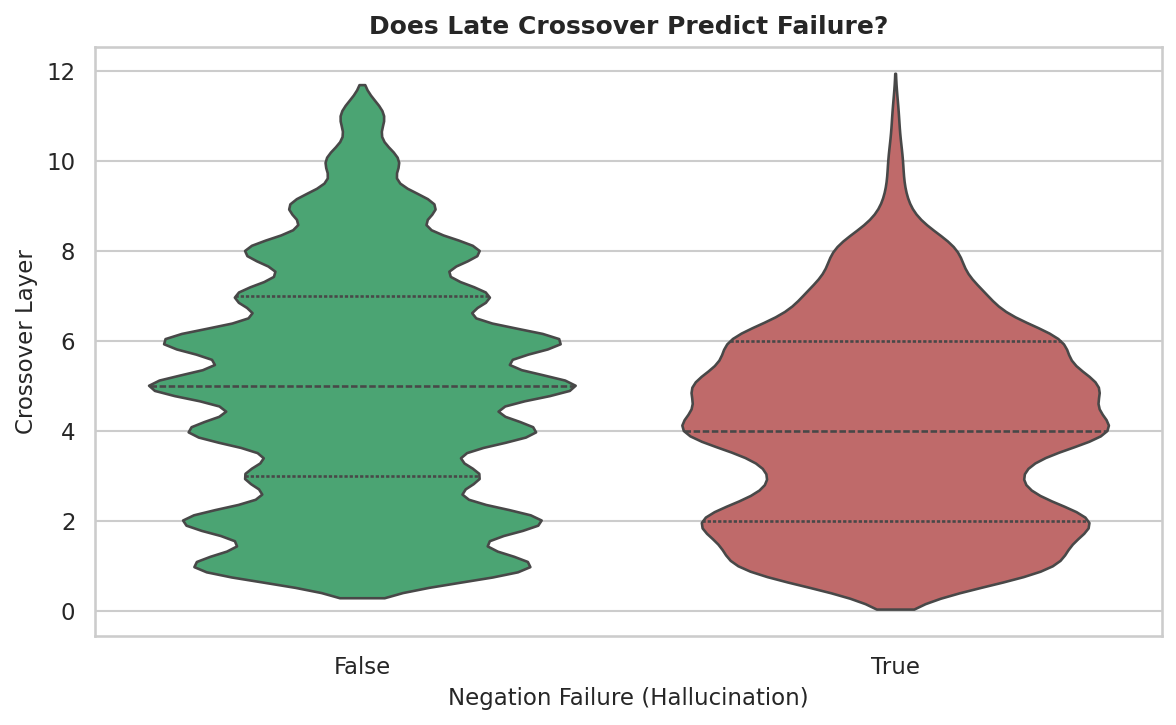
\includegraphics[width=\linewidth]{../../figures/cross_model/crossover_vs_failure.png}
  \caption{Crossover layer vs. negation outcome. Success cases cluster at layers 5--7; failures extend to layers 9--11 or lack a crossover entirely.}
  \label{fig:crossover_fail}
\end{figure}

\begin{itemize}
\item \textbf{Success cases} have crossover at layers 5--7 (Figure~\ref{fig:crossover_fail}).
\item \textbf{Failure cases} have late crossovers (layers 9--11) or no crossover at all (SGR~$= \infty$).
\item Crossover layer correlates inversely with SGR (Figure~\ref{fig:crossover_sgr}): early crossover $\Leftrightarrow$ low SGR $\Leftrightarrow$ successful suppression.
\end{itemize}

This establishes that the architecture has a \emph{window of opportunity}: if the inhibition circuit does not take control by the midpoint of the network, the factual signal becomes too deeply embedded in the residual stream to suppress.

\begin{figure}[t]
  \centering
  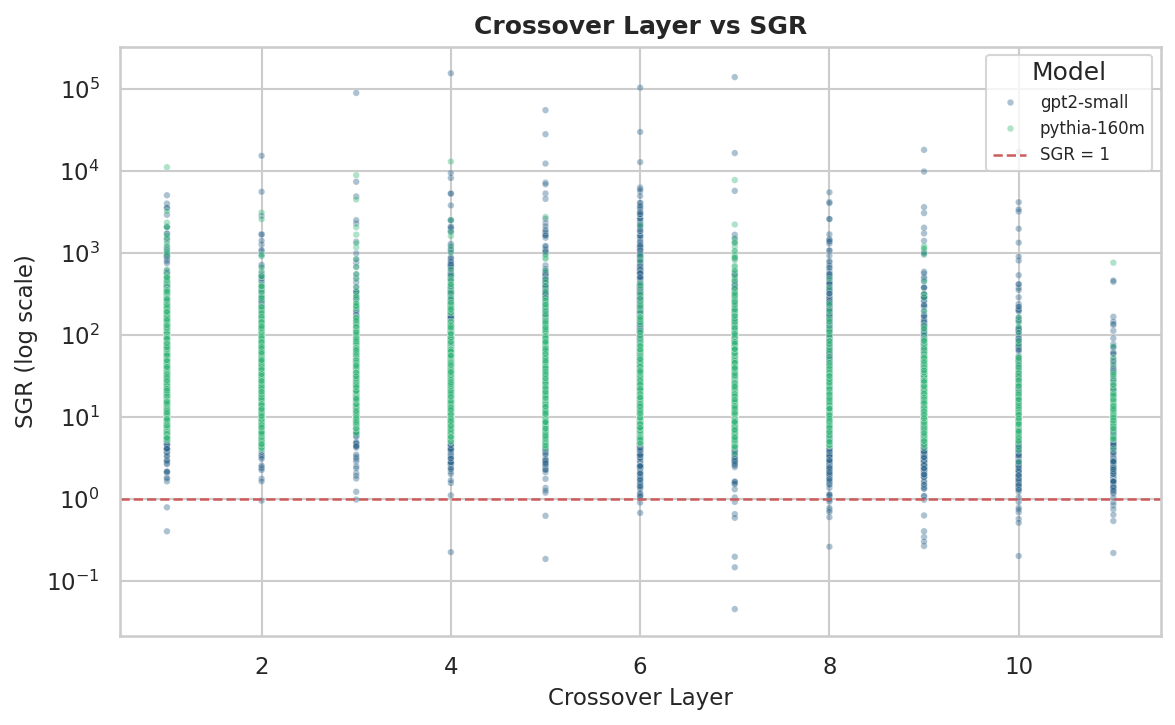
\includegraphics[width=\linewidth]{../../figures/cross_model/crossover_vs_sgr.png}
  \caption{Crossover layer vs. SGR (log scale). Early crossovers correspond to SGR\,$<$\,1; late crossovers map to extreme SGR values.}
  \label{fig:crossover_sgr}
\end{figure}

\subsection{Per-Head DLA and Inhibition Head Identification}

Per-head decomposition identifies the specific heads responsible for inhibition. For GPT-2 Small, the top-3 inhibition heads are $(9,8)$, $(10,0)$, and $(8,11)$, with mean $\Delta$DLA values of 5.59, 4.80, and 2.79 respectively (measured over 1,000 prompts). These heads consistently promote the target token on positive prompts but suppress it under negation, confirming their role as dedicated negation processors.

Across model families, inhibition heads scale proportionally with depth:

\begin{table}[h]
\centering\small
\begin{tabular}{@{}lc@{}}
\toprule
\textbf{Model} & \textbf{Top Inhibition Head} \\
\midrule
GPT-2 Small  & (9,\,8) layer 9  \\
GPT-2 Medium & (21,\,12) layer 21 \\
GPT-2 Large  & (30,\,6) layer 30  \\
Pythia-160M  & (9,\,4) layer 9  \\
Pythia-410M  & (17,\,6) layer 17 \\
\bottomrule
\end{tabular}
\caption{Top inhibition head by model. Inhibition concentrates in the final ${\sim}$25\% of layers across all scales.}
\label{tab:heads}
\end{table}

This consistent positioning at approximately 75--85\% depth suggests an architectural regularity: the inhibition circuit reliably forms in the late layers regardless of total depth.

\subsection{Activation Patching: Causal Evidence}
\label{sec:patching_results}

\begin{figure}[htbp]
  \centering
  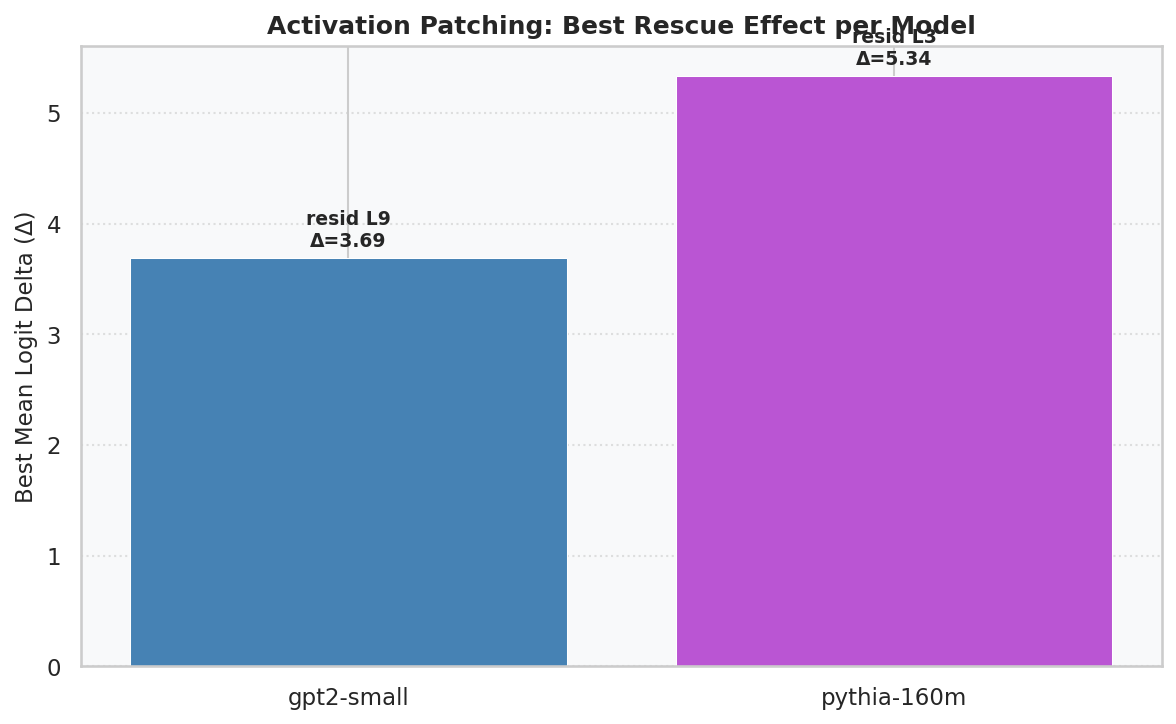
\includegraphics[width=\linewidth,height=0.85\textheight,keepaspectratio]{../../figures/cross_model/patching_summary.png}
  \caption{Activation patching rescue rates across all five models. Patching mid-layer attention outputs produces the highest rescue rates, causally confirming the inhibition circuit's localisation.}
  \label{fig:patching}
\end{figure}

We scaled activation patching to the full dataset, testing 1,000 samples per model and patching all three component types at every layer. Figure~\ref{fig:patching} shows the ``rescue rate'' the fraction of natural failures that are corrected by patching:

\begin{itemize}
\item \textbf{Early layers (0--4):} Patching has negligible effect. The inhibition circuit has not yet engaged.
\item \textbf{Mid layers (5--9):} Patching the \emph{attention stream} produces peak rescue rates. This is the causal confirmation that layers 5--9 contain the inhibition circuit.
\item \textbf{Late layers (10--11):} Rescue rates drop. The prediction is already committed.
\end{itemize}

This result provides the strongest \emph{causal} evidence in the project: supplying the model with ``correct logic'' exclusively within the mid-layer attention boundary is functionally equivalent to giving the entire model the correct logic for negation.

\subsection{Artificial Amplification}

\begin{figure}[htbp]
  \centering
  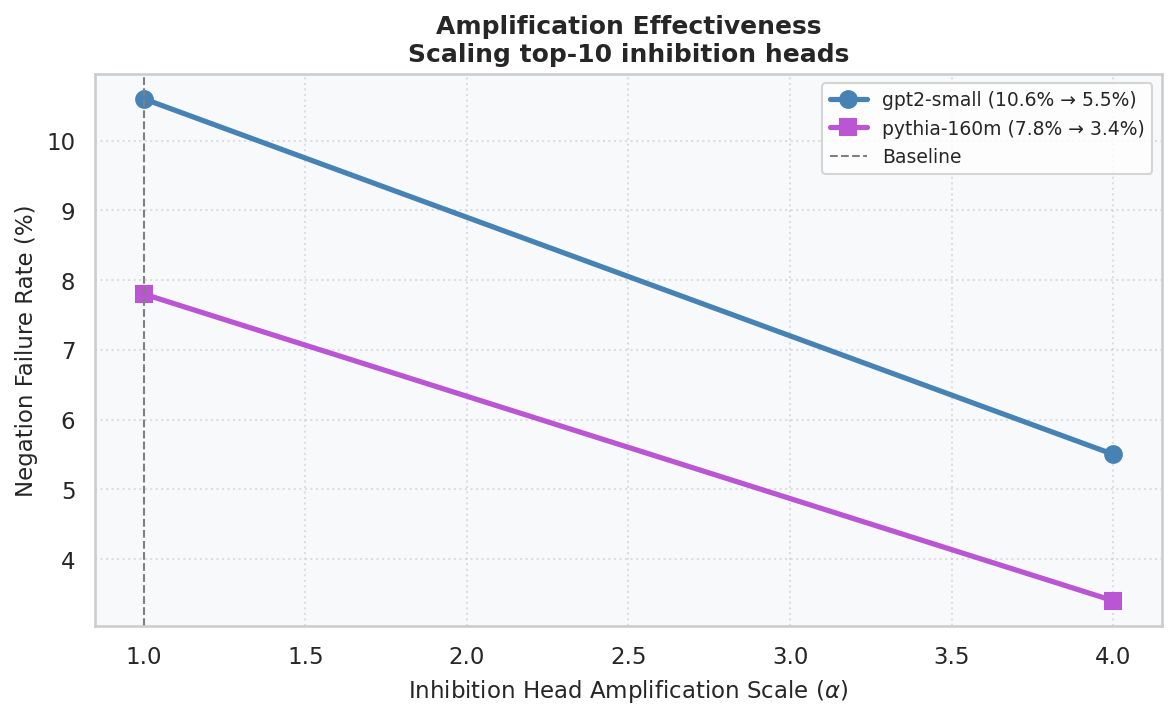
\includegraphics[width=\linewidth]{../../figures/cross_model/amplification_summary.png}
  \caption{Cross-model amplification comparison. Failure rates for all five models as a function of inhibition head amplification scale $\alpha$. The baseline ($\alpha\!=\!1$) is marked.}
  \label{fig:amp}
\end{figure}

Extended amplification experiments (Figure~\ref{fig:amp}) sweep finer scale grids ($\alpha \in \{1.0, 1.25, 1.5, 1.75, 2.0, 2.5, 3.0, 4.0\}$) across all five models:

\begin{table}[h]
\centering\small
\begin{tabular}{@{}lcccc@{}}
\toprule
\textbf{Model} & $\alpha\!=\!1$ & $\alpha\!=\!2$ & $\alpha\!=\!4$ & \textbf{Reduction} \\
\midrule
GPT-2 Small  & 10.4\% & 8.6\% & 5.5\%  & $-$47\% \\
GPT-2 Medium & 10.5\% & 10.2\% & 7.1\% & $-$32\% \\
GPT-2 Large  & 11.9\% & 13.0\% & 13.4\% & +13\% \\
Pythia-160M  & 7.6\%  & 7.8\% & 3.8\%  & $-$50\% \\
Pythia-410M  & 10.0\% & 9.3\% & 5.2\%  & $-$48\% \\
\bottomrule
\end{tabular}
\caption{Amplification effectiveness. Failure rate reduction at $\alpha\!=\!4$ vs.\ baseline. GPT-2 Large is the exception (\S\ref{sec:neg_results}).}
\label{tab:amp}
\end{table}

Key findings:

\paragraph{Amplification reduces failures causally.} For four out of five models, scaling the top-10 inhibition heads by $\alpha\!=\!4$ reduces negation failure by 32--50\%, confirming these heads' causal role in suppression.

\paragraph{Pythia responds more elastically.} Pythia-160M requires only $\alpha\!=\!1.75$ to begin showing clear reductions (7.6\%~$\to$~7.1\%), while GPT-2 Small requires $\alpha\!\geq\!2.0$ for meaningful effect. This suggests Pythia's inhibition heads are already closer to the suppression threshold.

\paragraph{GPT-2 Large is resistant.} GPT-2 Large shows \emph{increased} failure rates under amplification (discussed in \S\ref{sec:neg_results}).

\subsection{Semantic Vulnerability Audit}
\label{sec:audit}

We cross-referenced failure patterns with CounterFact's relation-type metadata to identify which \emph{kinds} of knowledge are structurally vulnerable to negation failure.

\paragraph{Extreme variance by relation type.} Failure rates range from 0\% to 83.3\% depending on the semantic relation:

\begin{itemize}
\item \textbf{Highly vulnerable:} ``field of work'' (83.3\%), ``languages spoken'' (60.0\%), ``official language'' (50.0\%). These are \emph{soft-associative} relations where multiple valid completions exist, and the model's FFN strongly encodes the most frequent association.
\item \textbf{Highly robust:} ``country of origin'' (0\%), ``position played'' (0\%), ``place of death'' (0\%). These are \emph{hard-categorical} relations where the target is uniquely defined.
\end{itemize}

\paragraph{The logit drop inversion.} In successful negation, the ``not'' token reduces the target logit by an average of 4.18 points. In \emph{failure} cases, the logit \emph{increases} by 1.04 points the negation paradoxically \emph{strengthens} the factual retrieval, exemplifying the Pink Elephant effect at the mechanistic level.



\paragraph{Subject complexity.} Multi-word subjects produce more failures (15 of 24 failures have $\geq$2-word subjects). Wider associative FFN activity for complex entities creates a stronger memory signal, making suppression harder.


\subsection{Qualitative Case Analysis}
\label{sec:qualitative}

To complement the dataset-scale quantitative results, we selected ten representative cases from the CounterFact benchmark evaluated on both GPT-2 Small and Pythia-160M, choosing cases that jointly exhibited: (i) strong negation-induced rank drops, (ii) cross-model failure disagreements, and (iii) SGR--failure mismatches. This diversity ensures the analysis spans both hard negation successes and failures.

\begin{figure}[htbp]
  \centering
  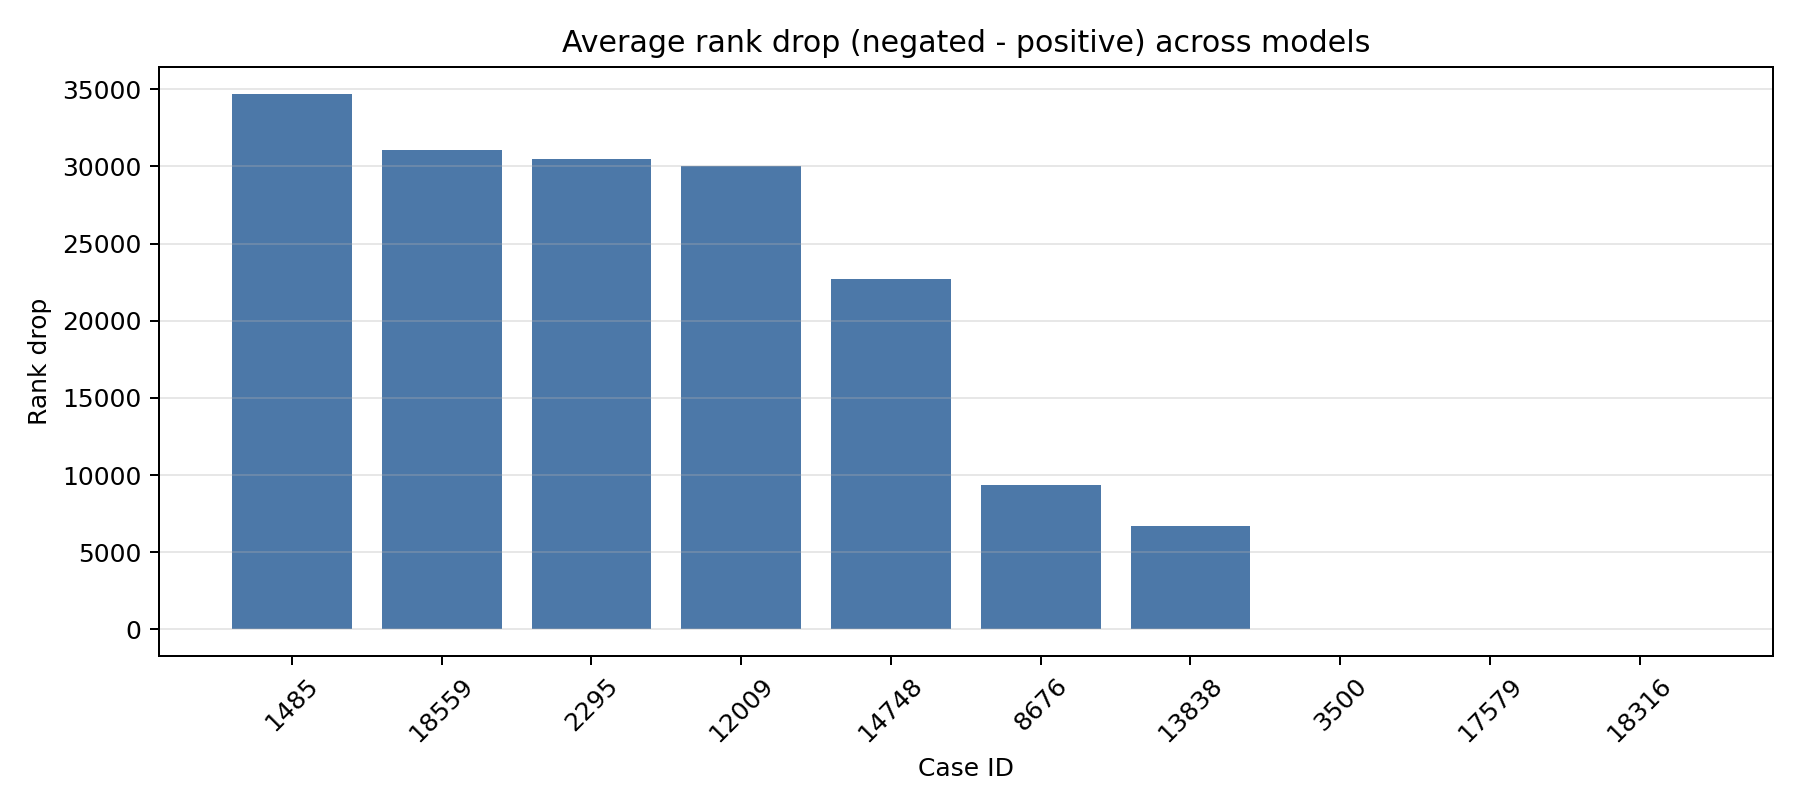
\includegraphics[width=\linewidth]{../../figures/qualitative/qualitative_case_comparison.png}
  \caption{Average rank drop (negated minus positive prompt) for the target token across the ten selected cases. Larger values indicate a stronger mechanistic response to negation, regardless of failure outcome.}
  \label{fig:qual_rank}
\end{figure}

\begin{figure}[htbp]
  \centering
  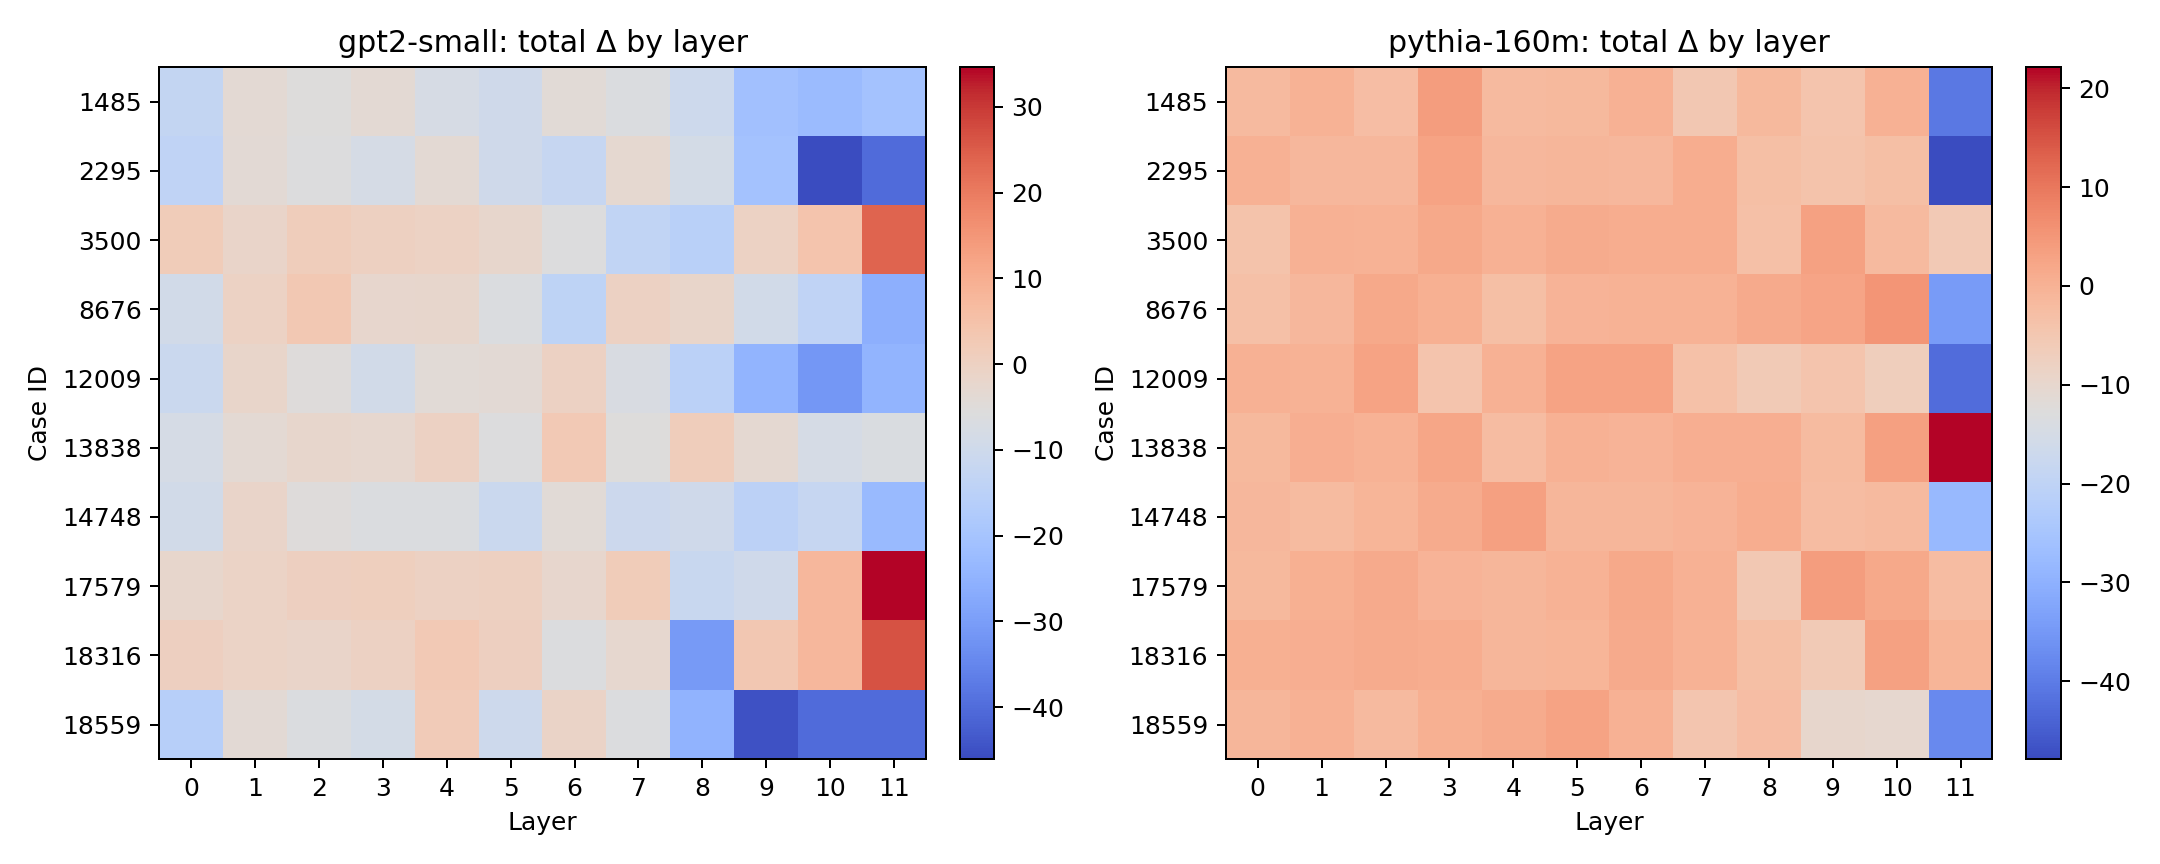
\includegraphics[width=\linewidth]{../../figures/qualitative/qualitative_layer_shift_heatmap.png}
  \caption{Layer-wise negation-induced shift ($\Delta$ contribution) heatmap for GPT-2 Small (left) and Pythia-160M (right). Each row is a selected case; each column is a transformer layer. Red indicates layers that paradoxically \emph{increase} target logit under negation; blue indicates effective suppression.}
  \label{fig:qual_heatmap}
\end{figure}

\paragraph{Rank drop is large even in successes.}
Figure~\ref{fig:qual_rank} shows that the average rank drop for the target token is substantial across all ten cases, including those where the model correctly avoided the factual completion. This confirms that ``not'' does alter the model's internal distribution, but the redirect often lands on a semantically similar token rather than a structurally distinct suppression.

\paragraph{Negation-induced shift is concentrated in late layers.}
Figure~\ref{fig:qual_heatmap} reveals a consistent pattern: the dominant shift layer for both models is concentrated in layer 10--11, with the top-3 layers accounting for 43--81\% of all absolute shift. This is fully consistent with our crossover analysis (Section~\ref{sec:results}), which locates the inhibition circuit at layers 5--9: the early layers \emph{detect} the negation signal, and the late layers deliver its cumulative suppression effect on the residual stream.

\paragraph{Inter-model disagreement reveals circuit brittleness.}
Several cases show failure on one model but success on the other (e.g.\ Case~8676 where GPT-2 Small succeeds at SGR$=0.012$ while Pythia-160M fails at SGR$=271$). These disagreements, absent in hard-categorical relations (geography, religion), concentrate in soft-associative relation types (occupation, language), corroborating the semantic audit findings in Section~\ref{sec:audit}.

% =================================================================
\section{Evaluation}

\label{sec:evaluation}
% =================================================================

\subsection{Hypothesis Validation}
Our experimental framework enables the direct evaluation of the Competitive Gating Hypothesis. Through the metrics outlined in our methodology, we assess the precise balance between FFN retrieval and attention inhibition.

The validation relies primarily on the Signal-to-Gate Ratio (SGR) and crossover layer metrics. When the inhibition signal exceeds retrieval (SGR\,$<$\,1), the model successfully suppresses the factual token. Correspondingly, crossover analysis and patching both converge on layers 5--9 as the critical boundary for 12-layer models. The systematic presence of this relationship confirms the core logic of the hypothesis.

% =================================================================
\section{Analysis}
\label{sec:analysis}
% =================================================================

\subsection{Positive Results}
\label{sec:pos_results}
Our framework generated multiple strong positive findings validating the mechanistic approach:
\begin{enumerate}
\item \textbf{SGR\,$<$\,1 is sufficient for success.} When the inhibition signal exceeds retrieval, the model never fails at negation (100\% success rate).
\item \textbf{FFN retrieval is logic-blind.} Mid-layer FFN DLA is essentially identical for positive and negated prompts, confirming that factual recall is context-independent.
\item \textbf{Amplification is causal.} Scaling inhibition heads reduces failure rates by up to 50\%, confirming their functional role.
\item \textbf{Semantic structure predicts failure.} Relations requiring soft-associative reasoning are mechanistically harder to inhibit than hard-categorical ones.
\end{enumerate}

\subsection{Negative Results}
\label{sec:neg_results}

\paragraph{GPT-2 Large resists amplification.} Uniquely among the five models, GPT-2 Large shows \emph{increased} failure rates when inhibition heads are amplified ($11.9\% \to 13.4\%$ at $\alpha\!=\!4$). We hypothesise that at 36 layers and 20 heads, the inhibition circuit is more distributed, and amplifying only 10 heads creates interference with the broader suppression ensemble. This suggests that the simple ``top-$k$ heads'' amplification strategy does not scale linearly with model depth.

\paragraph{Weak continuous correlations.} Spearman correlations between SGR and failure range from $r\!=\!0.008$ to $r\!=\!0.018$ for the larger models (Table~\ref{tab:stats}). This reflects a ceiling effect: when $>$83\% of samples have SGR\,$>$\,1, the metric's discriminative power operates primarily at its \emph{binary} threshold rather than as a continuous predictor.

\paragraph{Scaling does not help.} Counter to naive expectations, GPT-2 Large (774M params) fails \emph{more frequently} than GPT-2 Small (124M params). Larger FFN capacity amplifies retrieval without proportionally strengthening the inhibition circuit the memory muscle grows faster than the logic brake.

\subsection{Ablation Studies}
\label{sec:ablations}
While we leveraged activation patching to establish causal localization (Section \ref{sec:patching_results}) and artificial amplification to demonstrate causal sufficiency, we have not yet conducted formal network-wide ablation studies (e.g., iteratively removing or zeroing out individual inhibition heads). Activation patching provides a localized causal intervention, but comprehensive ablation tests will be necessary to confirm the strict \emph{necessity} of these identified heads across all contexts.

\subsection{Emotional Negation Geometry}
\label{sec:emotion}

To probe whether the negation failure mechanism extends beyond factual recall, we performed a complementary geometric analysis on \emph{emotional} prompts (anger, fear, joy, sadness) in GPT-2 Small and Pythia-160M using latent-space steering vectors.

\begin{figure}[htbp]
  \centering
  \begin{subfigure}[t]{0.48\linewidth}
    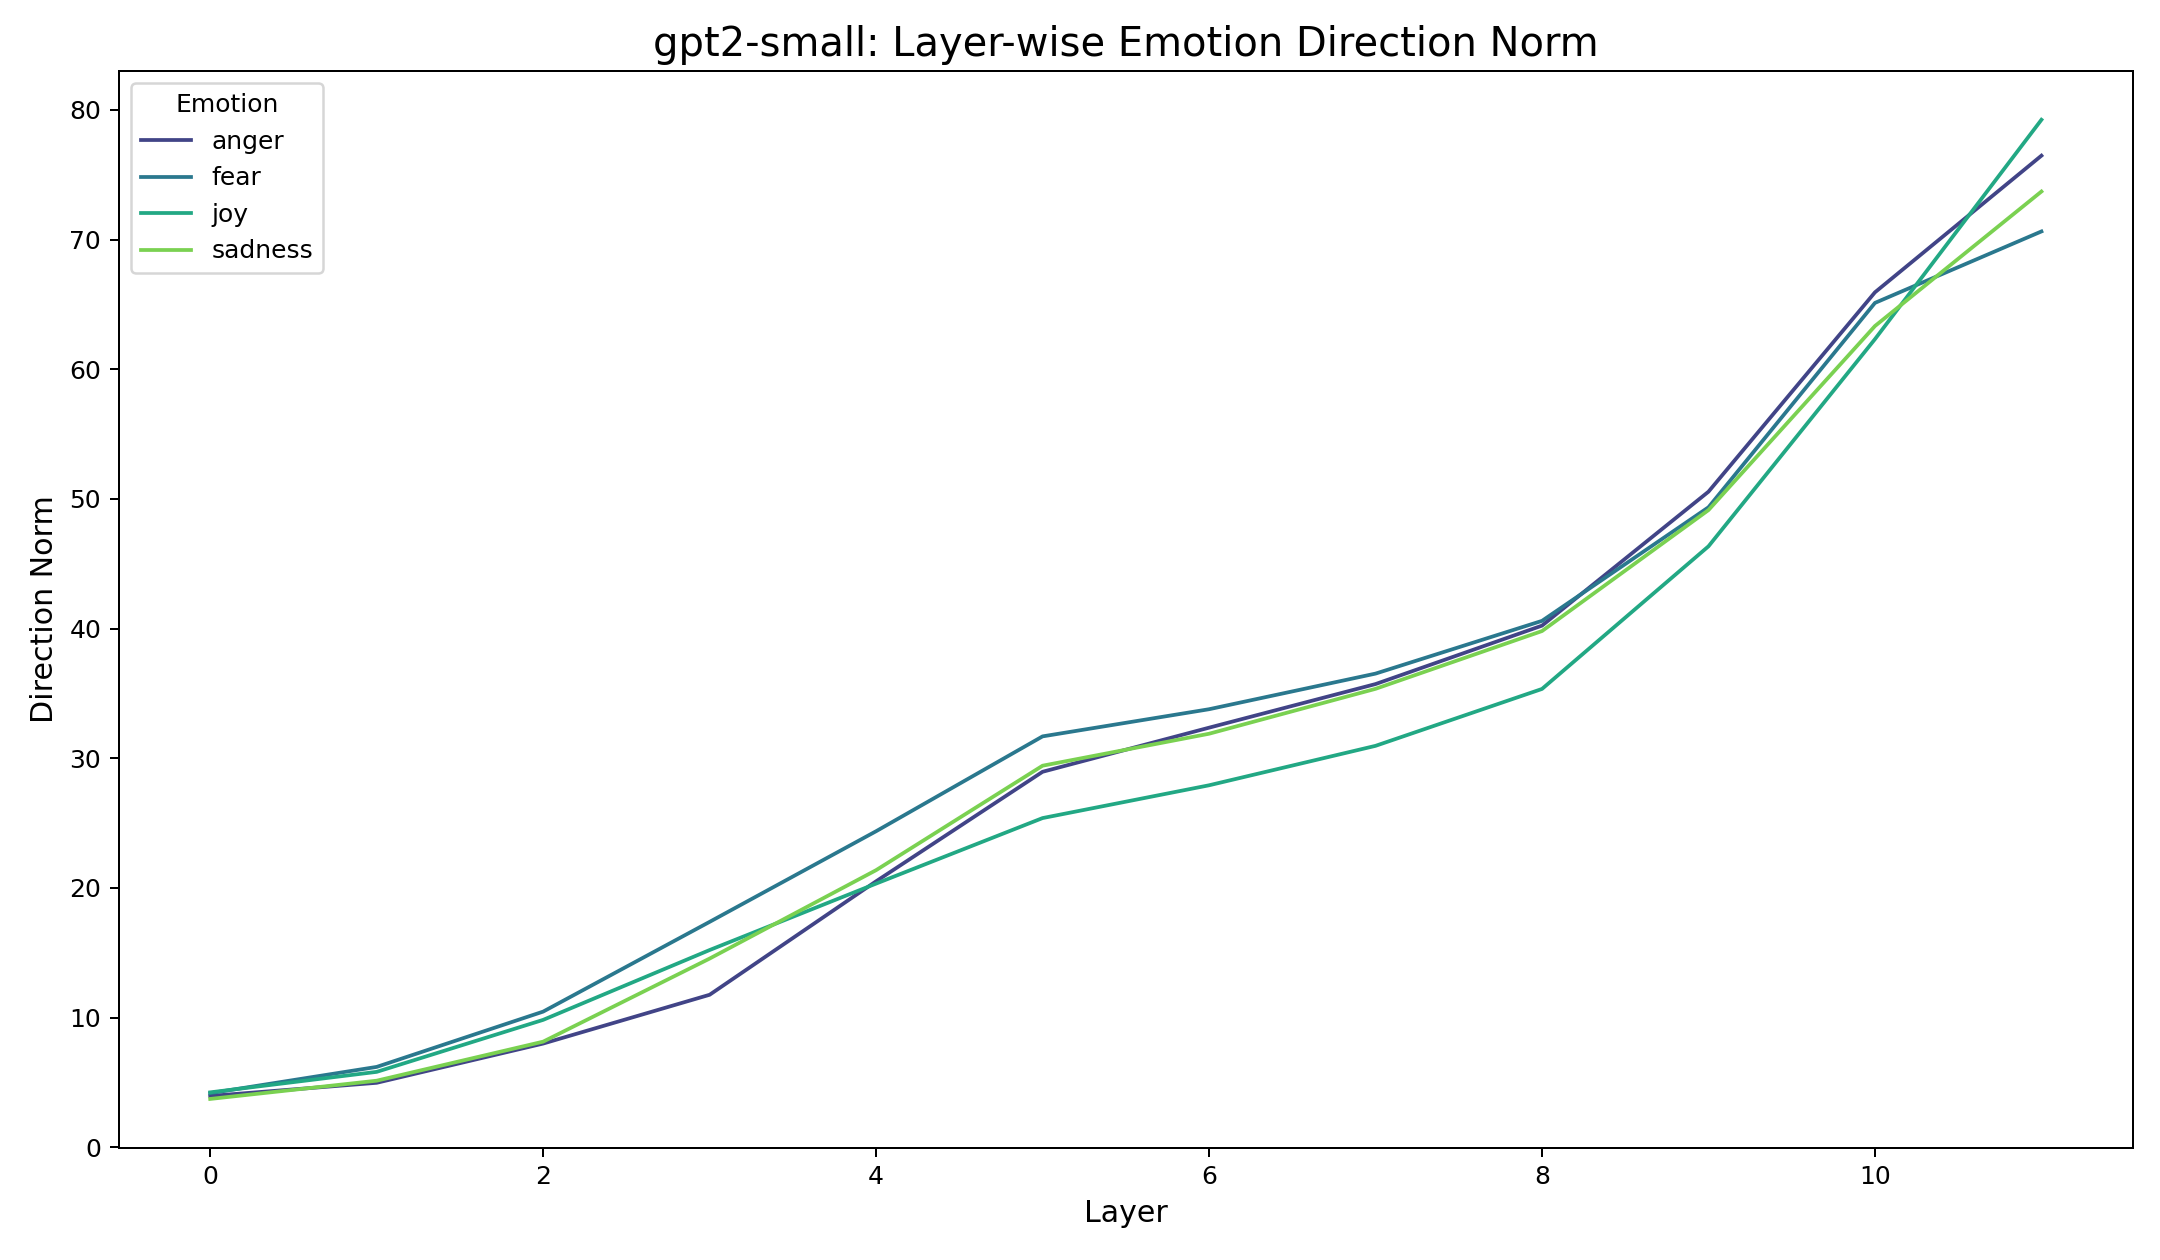
\includegraphics[width=\linewidth]{../../figures/emotion_negation/gpt2-small/layer_wise_direction_norm.png}
    \caption{GPT-2 Small}
  \end{subfigure}\hfill
  \begin{subfigure}[t]{0.48\linewidth}
    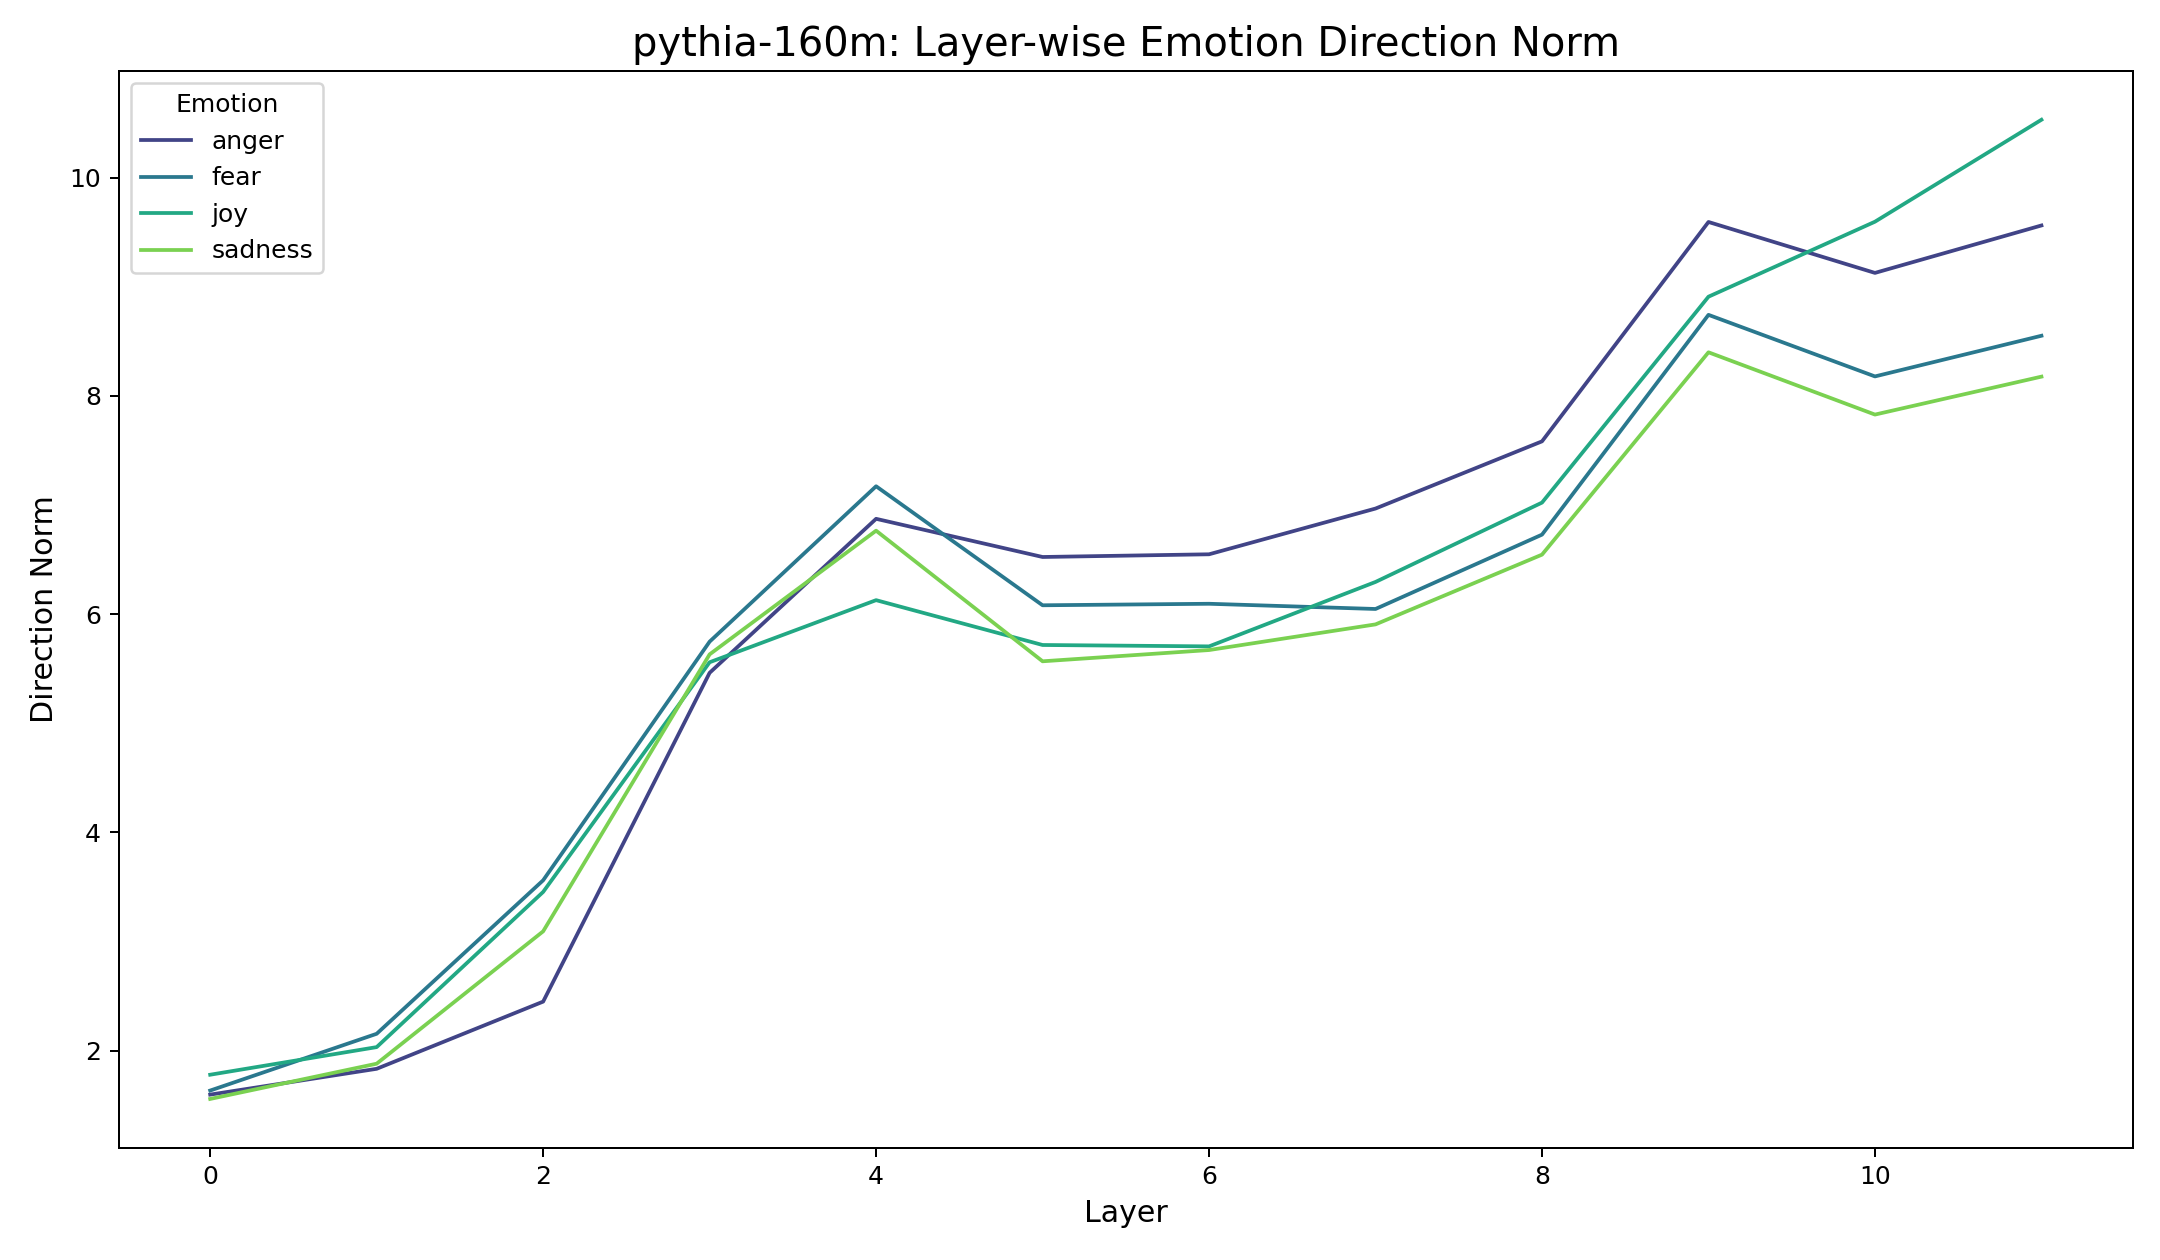
\includegraphics[width=\linewidth]{../../figures/emotion_negation/pythia-160m/layer_wise_direction_norm.png}
    \caption{Pythia-160M}
  \end{subfigure}
  \caption{Layer-wise emotional direction norm for four base emotions. GPT-2 Small peaks sharply at the final layer (L11); Pythia-160M peaks earlier and at lower magnitudes, reflecting architectural differences in residual scaling.}
  \label{fig:emotion_norm}
\end{figure}

\begin{figure}[htbp]
  \centering
  \begin{subfigure}[t]{0.48\linewidth}
    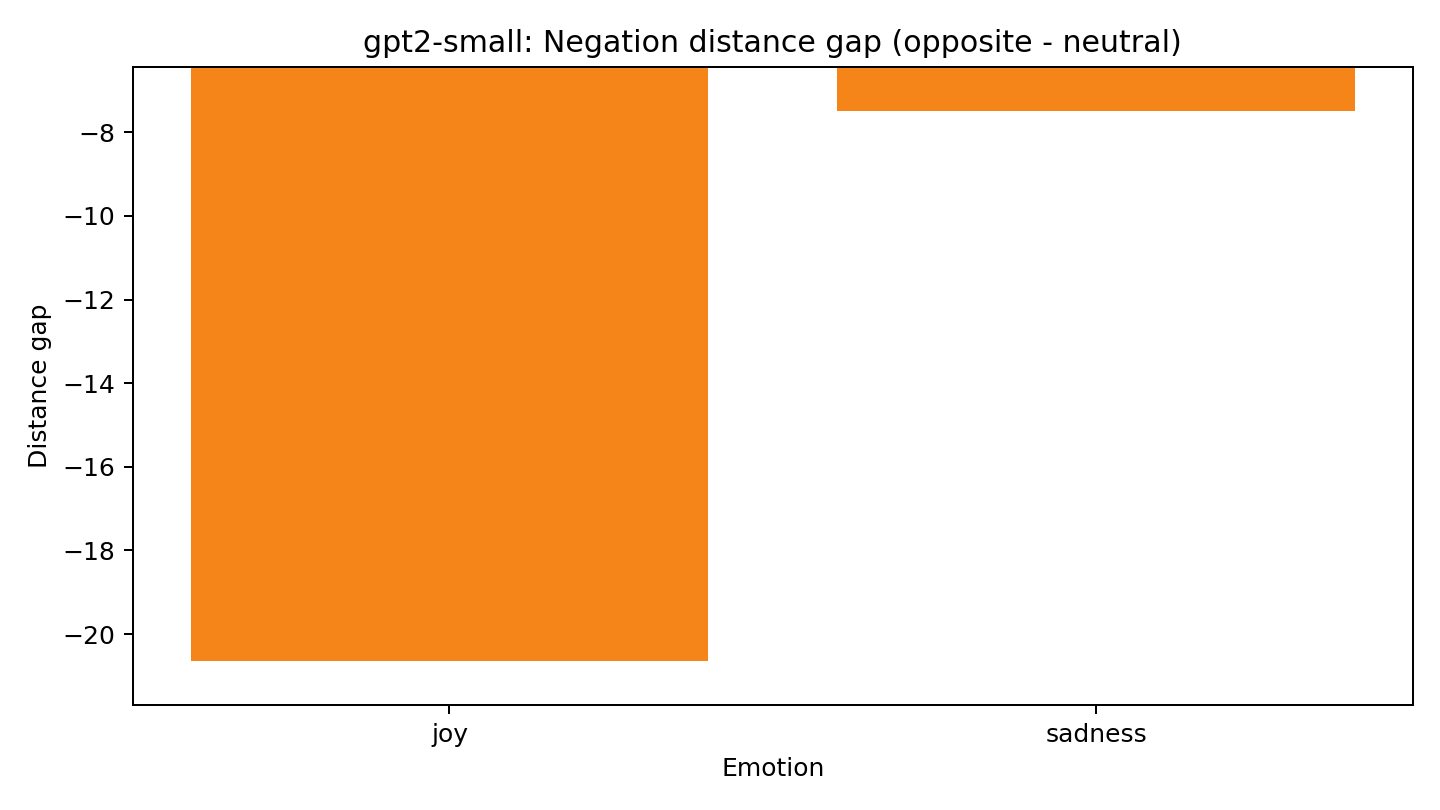
\includegraphics[width=\linewidth]{../../figures/emotion_negation/gpt2-small/negation_distance_gap.png}
    \caption{GPT-2 Small: distance gap}
  \end{subfigure}\hfill
  \begin{subfigure}[t]{0.48\linewidth}
    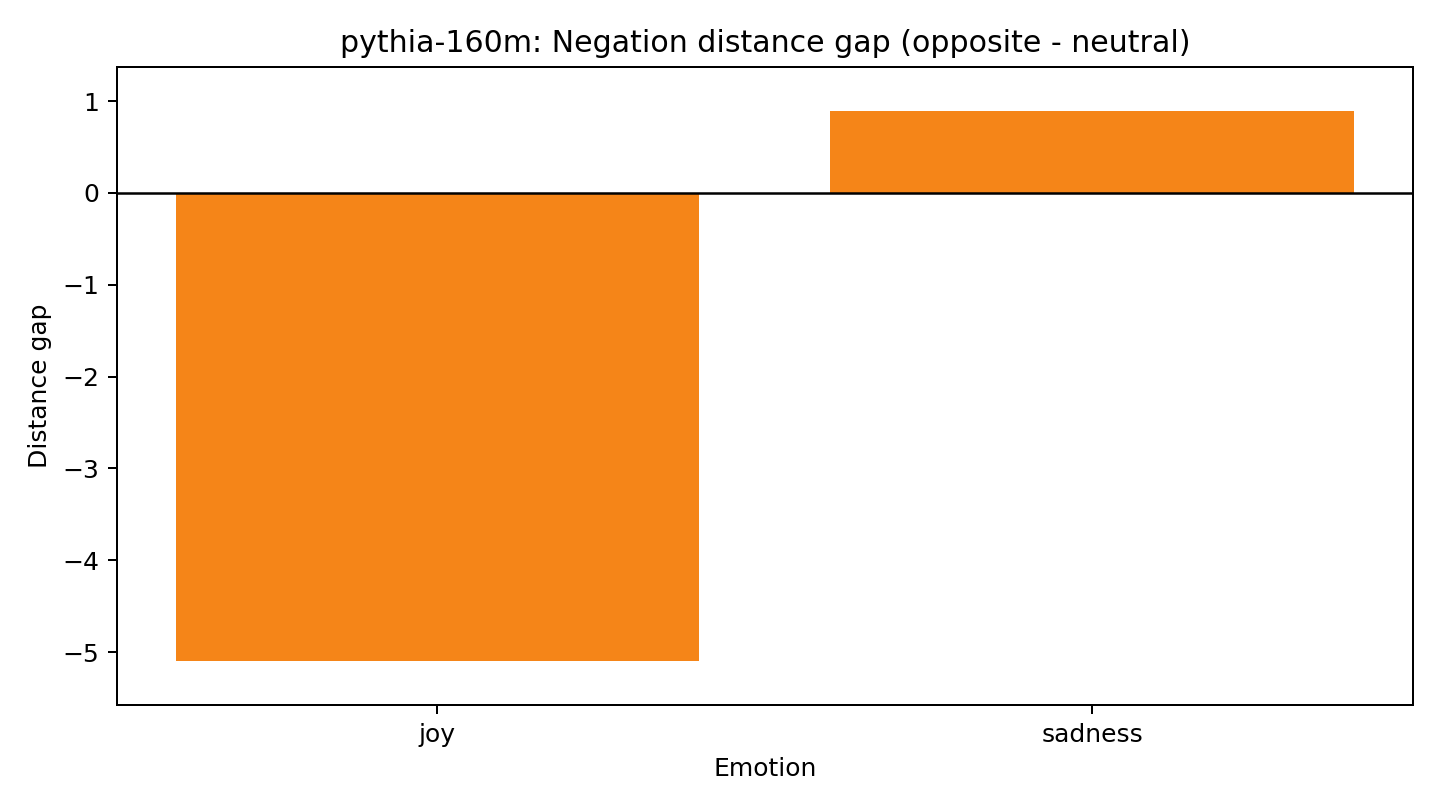
\includegraphics[width=\linewidth]{../../figures/emotion_negation/pythia-160m/negation_distance_gap.png}
    \caption{Pythia-160M: distance gap}
  \end{subfigure}
  \caption{Negation distance gap (distance-to-opposite minus distance-to-neutral). Negative values indicate the negated representation moves closer to the semantic opposite rather than to a neutral state.}
  \label{fig:emotion_gap}
\end{figure}

\paragraph{Emotional features solidify in late layers.}
As shown in Figure~\ref{fig:emotion_norm}, GPT-2 Small peaks at L11 (norms 70.6--79.2), while Pythia-160M peaks earlier (L9 for anger/fear/sadness) with lower magnitudes ($\sim$8.4--10.5). This mirrors our factual-recall findings: high-level semantic concepts require the full transformer depth to crystallise in the residual stream, consistent with the FFN-as-key-value-memory framework \cite{geva-etal-2021-transformer}.

\paragraph{Residual stream expansion confirms deep encoding.}
Both models show a large norm increase from early to late layers (GPT-2 Small: ${\sim}13\to50$; Pythia-160M: ${\sim}4\to8$). This matches the \emph{logit lens} framework: the model accumulates emotional evidence across layers, reaching semantic saturation just before unembedding.

\paragraph{Negation induces crude geometric inversion, not logical flip.}
Figure~\ref{fig:emotion_gap} shows that in GPT-2 Small, negated joy/sadness prompts yield negative distance gaps, meaning the representation moves toward the \emph{semantic opposite} rather than toward a neutral state. This is a geometric analogue of the Pink Elephant effect: ``not joy'' is encoded as ``sadness,'' not ``neutral,'' because the model focuses on the emotion's topic rather than its logical complement.

\paragraph{Pythia-160M defaults to neutral on negation.}
Pythia-160M exhibits a positive gap for sadness (0.88), meaning ``not sad'' converges to a neutral rather than a joyful state. This \emph{unipolar} representation suggests Pythia lacks the contrastive latent geometry GPT-2 uses for emotional inversion, consistent with higher closer-to-neutral rates (Joy: 0.22, Sadness: 0.77 vs.\ 0.0/0.20 for GPT-2 Small).

\paragraph{Emotion linearity is emotion-specific.}
Intervention $R^2$ values are high for most emotion--model pairs (anger/fear/sadness in GPT-2: $R^2\approx0.90$--$0.97$; fear/joy/sadness in Pythia: $R^2>0.87$), confirming the Linear Representation Hypothesis for those emotions. The outliers---joy in GPT-2 Small ($R^2=0.22$) and anger in Pythia-160M ($R^2=0.28$)---suggest those emotions are encoded as multi-modal or non-linear manifolds, likely due to their higher polysemy.

\paragraph{Intervention slopes are near-zero across all emotions.}
Despite high $R^2$, slopes are extremely small (${\sim}10^{-4}$), indicating the emotional steering direction is approximately orthogonal to the model's primary next-token prediction pathway. Changing emotional representations in the residual stream requires large-magnitude interventions to shift output behaviour---consistent with activation-addition findings and the strong FFN retrieval dominance observed in our factual negation experiments.

\subsection{Soft Negation Variants}
\label{sec:soft_negation}

We extended the pipeline to test three additional negation constructions---\textit{``unlikely to be''}, \textit{``rarely''}, and \textit{``maybe''}---against the hard \textit{``not''} baseline across GPT-2 Small and Pythia-160M on the full CounterFact dataset. This tests whether the Competitive Gating Hypothesis generalises beyond single-token negation.

\begin{table}[htbp]
\centering\small
\begin{tabular}{@{}llrrrr@{}}
\toprule
\textbf{Model} & \textbf{Negator} & \textbf{Fail\,\%} & \textbf{Med.\,SGR} & \textbf{SGR$>$1\,\%} \\
\midrule
\multirow{4}{*}{GPT-2 Small}
  & not (hard)        & 11.40 & 27.1 & 99.1 \\
  & unlikely to be    &  4.51 & 17.3 & 91.3 \\
  & rarely            &  \textbf{2.93} &  \textbf{9.7} & 84.2 \\
  & maybe             &  9.08 & 41.1 & 99.4 \\
\midrule
\multirow{4}{*}{Pythia-160M}
  & not (hard)        &  9.02 & 24.5 & 100.0 \\
  & unlikely to be    &  3.98 & 22.9 &  99.8 \\
  & rarely            &  \textbf{3.52} & 25.4 &  99.9 \\
  & maybe             &  9.18 & 35.0 &  99.9 \\
\bottomrule
\end{tabular}
\caption{Failure rates and SGR statistics across four negation constructions. \textit{Rarely} achieves the lowest failure rate for both models.}
\label{tab:soft_neg}
\end{table}

\begin{figure}[htbp]
  \centering
  \begin{subfigure}[t]{0.48\linewidth}
    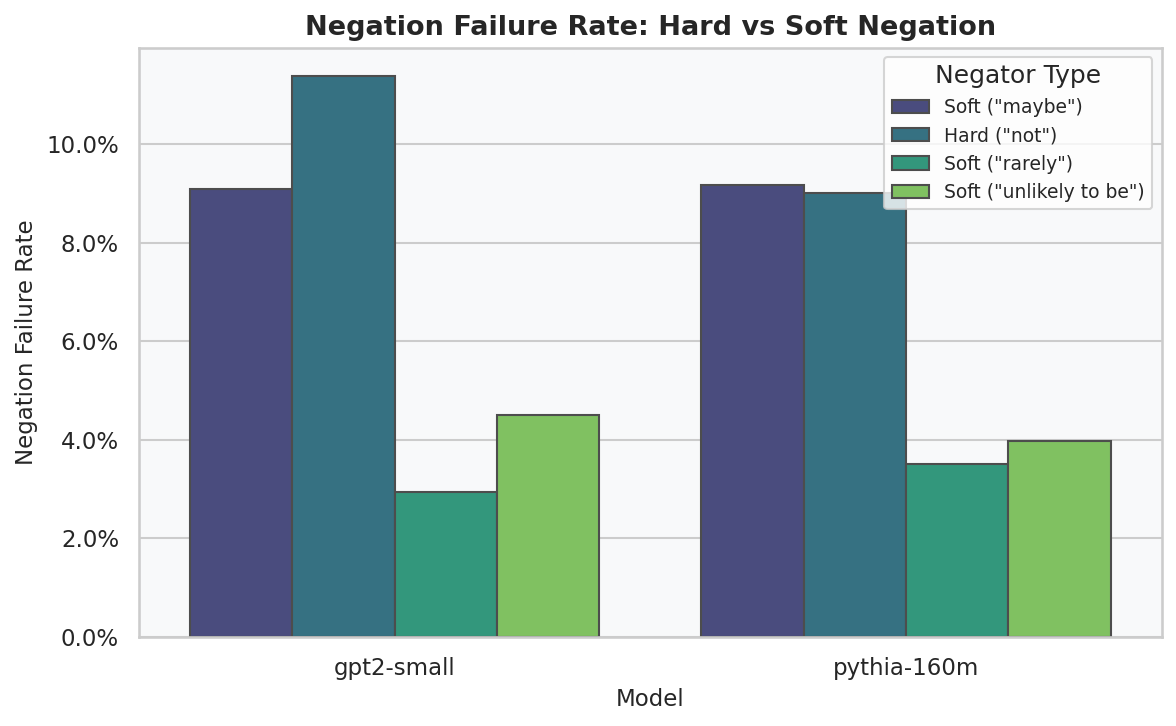
\includegraphics[width=\linewidth]{../../figures/soft_negation/failure_rate_comparison.png}
    \caption{Failure rate per negator}
  \end{subfigure}\hfill
  \begin{subfigure}[t]{0.48\linewidth}
    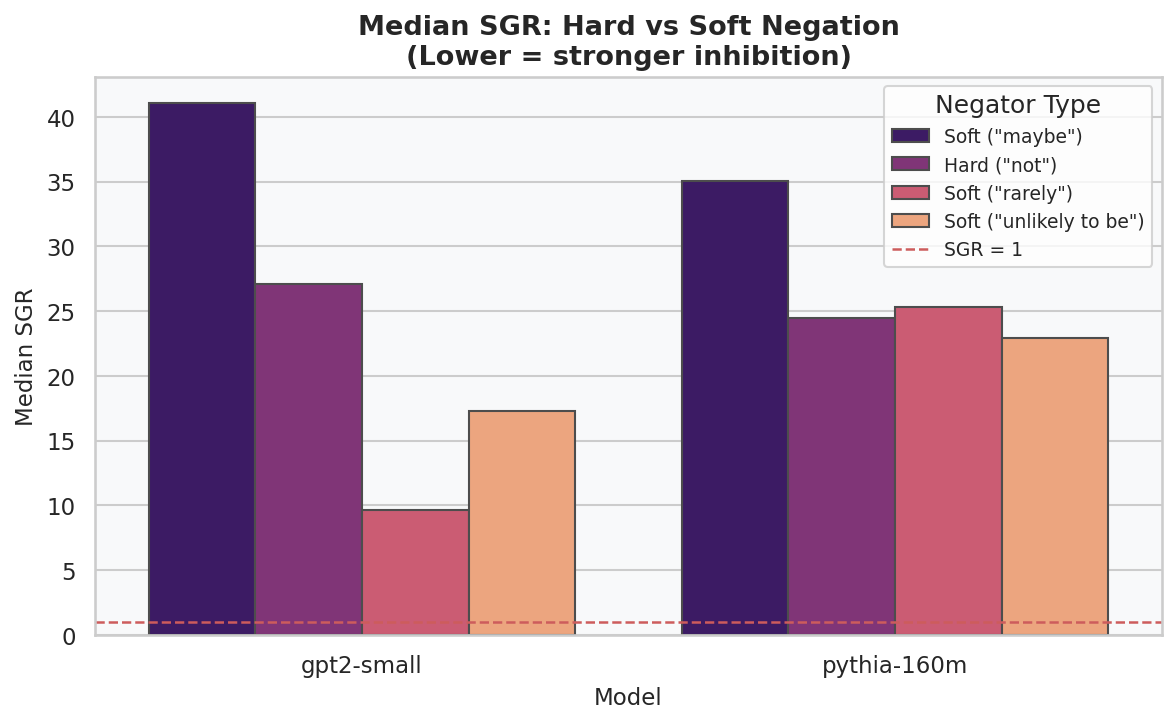
\includegraphics[width=\linewidth]{../../figures/soft_negation/median_sgr_comparison.png}
    \caption{Median SGR per negator}
  \end{subfigure}
  \caption{Soft negation comparison across models. \textit{Rarely} and \textit{unlikely to be} consistently outperform hard \textit{not} on both failure rate and median SGR.}
  \label{fig:soft_neg}
\end{figure}

\paragraph{Soft negators outperform hard negation (hypothesis partially rejected).}
Our pre-experiment prediction was that soft negators would produce \emph{weaker} inhibition than hard ``not.'' The data refutes this for \textit{rarely} and \textit{unlikely to be}: \textit{rarely} reduces failure rates from 11.4\% to 2.9\% in GPT-2 Small and from 9.0\% to 3.5\% in Pythia-160M---a larger reduction than any amplification experiment achieved natively. This shows the inhibition circuit is sensitive to semantic content, not just the literal ``not'' token.

\paragraph{Lower SGR under soft negation implicates retrieval reduction.}
For GPT-2 Small, the median SGR drops from 27.1 (hard) to 9.7 (\textit{rarely}). Since $\text{SGR} = \text{FFN retrieval} / \text{Attn inhibition}$, the drop could reflect stronger inhibition or weaker retrieval. Given that \textit{rarely} and \textit{unlikely to be} are multi-word, low-frequency suffixes in the training corpus, we hypothesise the FFN encodes weaker factual associations for these constructions, reducing retrieval strength and making the inhibition circuit's task substantially easier.

\paragraph{\textit{Maybe} as a control validates the pipeline.}
\textit{Maybe} is an ambiguity marker, not a logical negation. Its failure rate (9.1\% / 9.2\%) is nearly identical to hard negation, and its median SGR is the \emph{highest} of all four negators, confirming that the model's inhibition circuit does not engage under ambiguous constructions. This control validates our pipeline: it correctly detects the absence of a suppressive signal.

\paragraph{SGR boundary holds for soft negators with one exception.}
Across all negators, SGR\,$<$\,1 continues to yield zero failures---except for \textit{rarely} in GPT-2 Small, where 14 failures occur at SGR\,$\leq$\,1 (2.18\% of failures). This single breakdown suggests \textit{rarely} occasionally recruits a qualitatively different circuit pathway that the FFN/Attention DLA split does not fully capture, motivating future head-level analysis.

\subsection{Limitations and Challenges}
\label{sec:limitations}



\begin{itemize}
\item \textbf{Hard negation focus.} The main benchmark uses ``is not'' negation. Soft constructions (``unlikely to be,'' ``rarely'') were tested as an extension (Section~\ref{sec:soft_negation}) and show substantially lower failure rates, but head-level DLA for these negators remains future work.
\item \textbf{Single dataset.} All results use CounterFact. Generalisation to free-form negation in open-ended generation remains untested.
\item \textbf{SGR\,$<$\,1 rarity.} The perfect success rate at SGR\,$<$\,1 is based on very few samples ($n\!=\!1$ for GPT-2 Small's finite-SGR samples). While promising, larger sample sizes at this threshold are needed for stronger claims.
\item \textbf{Top-$k$ head selection.} Our amplification strategy amplifies a fixed set of 10 heads. The GPT-2 Large results suggest this may be too coarse for deeper models.
\item \textbf{Causal granularity.} Patching at the layer level conflates multiple head contributions. Head-level patching would provide finer causal resolution.
\end{itemize}

\subsection{Ethics Statement}

This work analyses the internal mechanisms of publicly available language models (GPT-2, Pythia) using an established public dataset (CounterFact). No private data, personal information, or sensitive content is involved. Our findings about negation failure could inform alignment research by identifying specific architectural components that require strengthening for safer model deployment.

\subsection{Future Work}

\begin{itemize}
\item \textbf{Soft negation:} Extend to ``is unlikely to be'' and ``rarely'' constructions, comparing SGR distributions to hard negation.
\item \textbf{Head-level patching:} Patch individual inhibition heads rather than full layers for finer causal resolution.
\item \textbf{Ablation:} Remove individual inhibition heads to confirm causal \emph{necessity} (complementing the amplification sufficiency evidence).
\item \textbf{Larger models:} Test on GPT-2 XL, Pythia-1B, and instruction-tuned models to determine whether RLHF strengthens the inhibition circuit.
\item \textbf{Free-form negation:} Evaluate on open-ended generation tasks beyond the structured CounterFact format.
\end{itemize}

% =================================================================
\section{Conclusion}
\label{sec:conclusion}
% =================================================================

We presented the Competitive Gating Hypothesis that negation failure in LLMs arises from a mechanistic imbalance between automatic factual retrieval (FFNs) and late-stage logical inhibition (attention heads) and provided comprehensive empirical support across five transformer models totalling over 80,000 evaluation points.

The Signal-to-Gate Ratio (SGR) emerged as a powerful diagnostic metric: SGR\,$<$\,1 perfectly predicts negation success, and SGR\,$>$\,1 is a necessary condition for all observed failures. Crossover analysis pinpointed the critical inhibition boundary at layers 5--7 for 12-layer models, and activation patching causally confirmed that this boundary hosts the inhibition circuit. Artificial amplification reduced failure rates by up to 50\%, and semantic auditing revealed that soft-associative relations are systematically more vulnerable than hard-categorical ones.

Our results have implications beyond negation: any task requiring a transformer to \emph{override} its most probable completion faces the same retrieval--inhibition bottleneck. The Competitive Gating Hypothesis provides a framework for understanding and potentially mitigating this class of failures.


% =================================================================
% References
% =================================================================
\bibliography{references}

\end{document}
